\RequirePackage[T1]{fontenc}
\documentclass[letterpaper,10pt,conference]{ieeeconf}
\IEEEoverridecommandlockouts
\overrideIEEEmargins
\usepackage{amsmath,amssymb,graphicx,booktabs,url,xcolor,tikz,balance}
\usetikzlibrary{arrows.meta,positioning}
\usepackage[hidelinks]{hyperref}
% Generated from the immutable partial development snapshot.
\newcommand{\SCVerified}{6}
\newcommand{\SCAttempts}{7}
\newcommand{\SCEligible}{6}
\newcommand{\SCMedianSim}{30.11}
\newcommand{\SCMedianWall}{282.7}
\newcommand{\SCPeakForce}{3.32}
\newcommand{\SCInterval}{61.0--100.0}
\newcommand{\SFPVerified}{5}
\newcommand{\SFPAttempts}{7}
\newcommand{\SFPEligible}{6}
\newcommand{\SFPMedianSim}{58.05}
\newcommand{\SFPMedianWall}{561.1}
\newcommand{\SFPPeakForce}{3.29}
\newcommand{\SFPInterval}{43.6--97.0}

\title{Visual and Contact Registration for Last-Inch\\SC and SFP Connector Insertion}
\author{Working draft for author review}
\newcommand{\pending}[1]{\textit{[Results pending: #1]}}
\begin{document}
\maketitle
\thispagestyle{plain}\pagestyle{plain}

\begin{abstract}
Reliable connector insertion requires correcting the errors that sensors can
actually observe near an occluded mating surface. We extend an existing
confidence-weighted multiview perception pipeline with connector-specific
relative contact registration: an optical connector uses its terminal shoulder,
whereas a small form-factor pluggable module uses opposed entrance-lip and
side-wall measurements. Bounded impedance-control targets carry the resulting
corrections through insertion. We evaluate the held-grasp, upstream-aligned
last-inch task in headless Gazebo using public challenge geometry and an
independent geometry, contact, and full-rate force recorder. A frozen partial
development snapshot contains six verified optical-connector seats in six
policy trials and five verified module seats in six policy trials; one
additional module setup failed before execution. All completed policy trials
have complete 2,000 Hz force coverage, with a maximum raw tared force of
3.322 N. A module perception rejection and a controller
startup failure remain in the record. The evidence demonstrates conditional
insertion capability and exposes timing and observability failures; broader
robustness and current-method causal comparisons remain under evaluation.
\end{abstract}

\begin{keywords}
Robotic assembly, connector insertion, visual perception, contact sensing,
simulation evaluation.
\end{keywords}

\section{Application and scope}
SC optical connectors and small form-factor pluggable (SFP) modules present
different mating geometries despite sharing a familiar align-and-insert task.
Near engagement, the gripper and connector obscure useful image features, and
compliant robot tracking can leave residual errors after a valid pose command.
Our starting point is a challenge pipeline that combines learned landmarks,
confidence-weighted multiview reconstruction, a visually estimated grasp
transform, and force-aware insertion~\cite{team}. We retain that perception
structure and isolate the final insertion skill for inspection in Gazebo.

The task begins with a connector held rigidly near the requested port.
Upstream angular alignment is prescribed; translation and the in-hand offset
are estimated from images. The policy preserves the handed-off wrist
orientation. SC angular perturbations have components within $\pm0.1^\circ$;
SFP uses $\pm0.03^\circ$ and a public level-fixture prior. Seeded in-hand
translation can vary by $\pm2$ mm per component. These conditions define
conditional last-inch insertion, excluding pickup, long-range transport,
unrestricted rotational recovery, and release retention.

Related work already establishes the main ingredients. Active Extrinsic
Contact Sensing estimates external contacts to guide insertion~\cite{kim2022}.
Insert-One combines visual tracking with impedance control under in-hand pose
uncertainty~\cite{chang2024}. SyPAS uses synthetic socket perception and visual
servoing before compliant connector insertion~\cite{sypas}; FORGE learns
force-aware manipulation under pose uncertainty~\cite{noseworthy2024}.
Factory and IndustReal address contact-rich simulation and transfer,
respectively~\cite{narang2022,tang2023}. We do not claim these general principles
as new, or compare success rates across their different tasks.

The practical contribution examined here is the allocation of uncertain
relative coordinates to connector-specific measurements. Image geometry
initializes alignment; qualified physical datums correct unresolved axial or
lateral bias; a separate evaluator determines whether a seat occurred.
Figure~\ref{fig:camera} shows the actual source meshes. The candidate advantage
of this allocation, beyond feasibility, requires matched current-method
ablations that are still pending.

\begin{figure}[t]
\centering
\begin{tabular}{@{}c@{\hspace{.02\columnwidth}}c@{}}
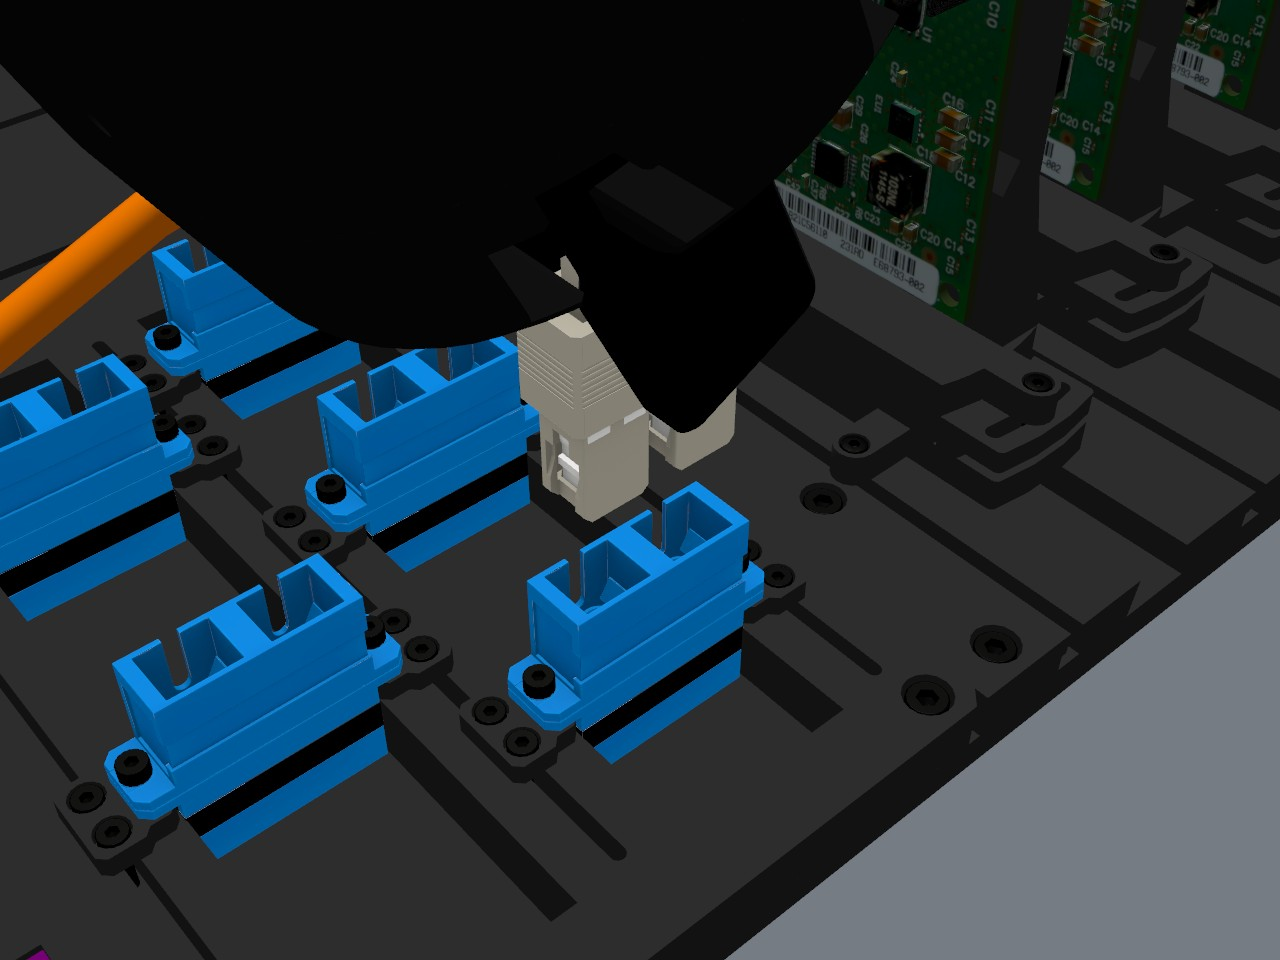
\includegraphics[width=.485\columnwidth]{figures/sc_before.jpg}&
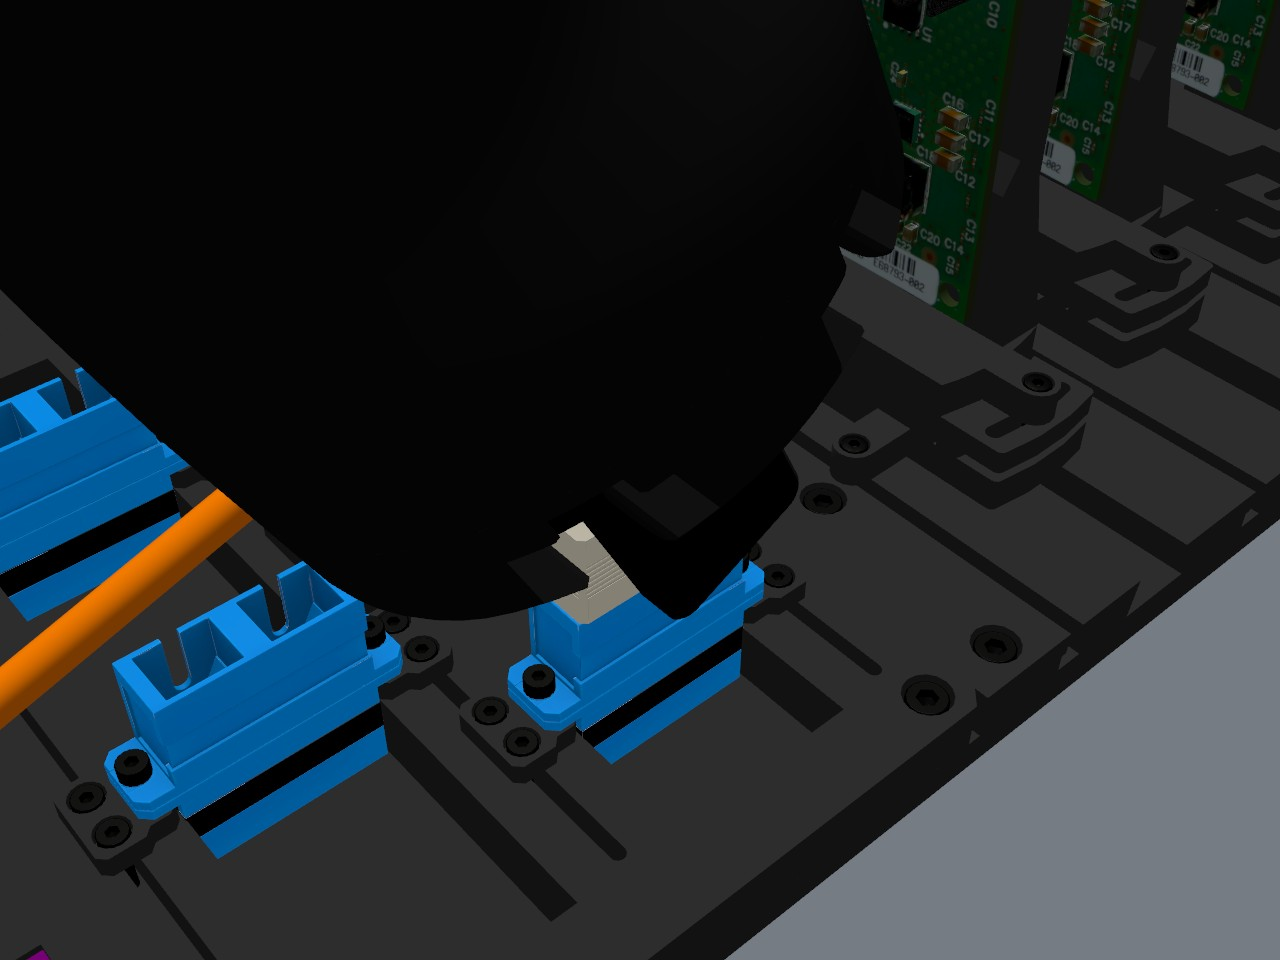
\includegraphics[width=.485\columnwidth]{figures/sc_after.jpg}\\[-2pt]
\scriptsize SC approach&\scriptsize SC verified seat\\[3pt]
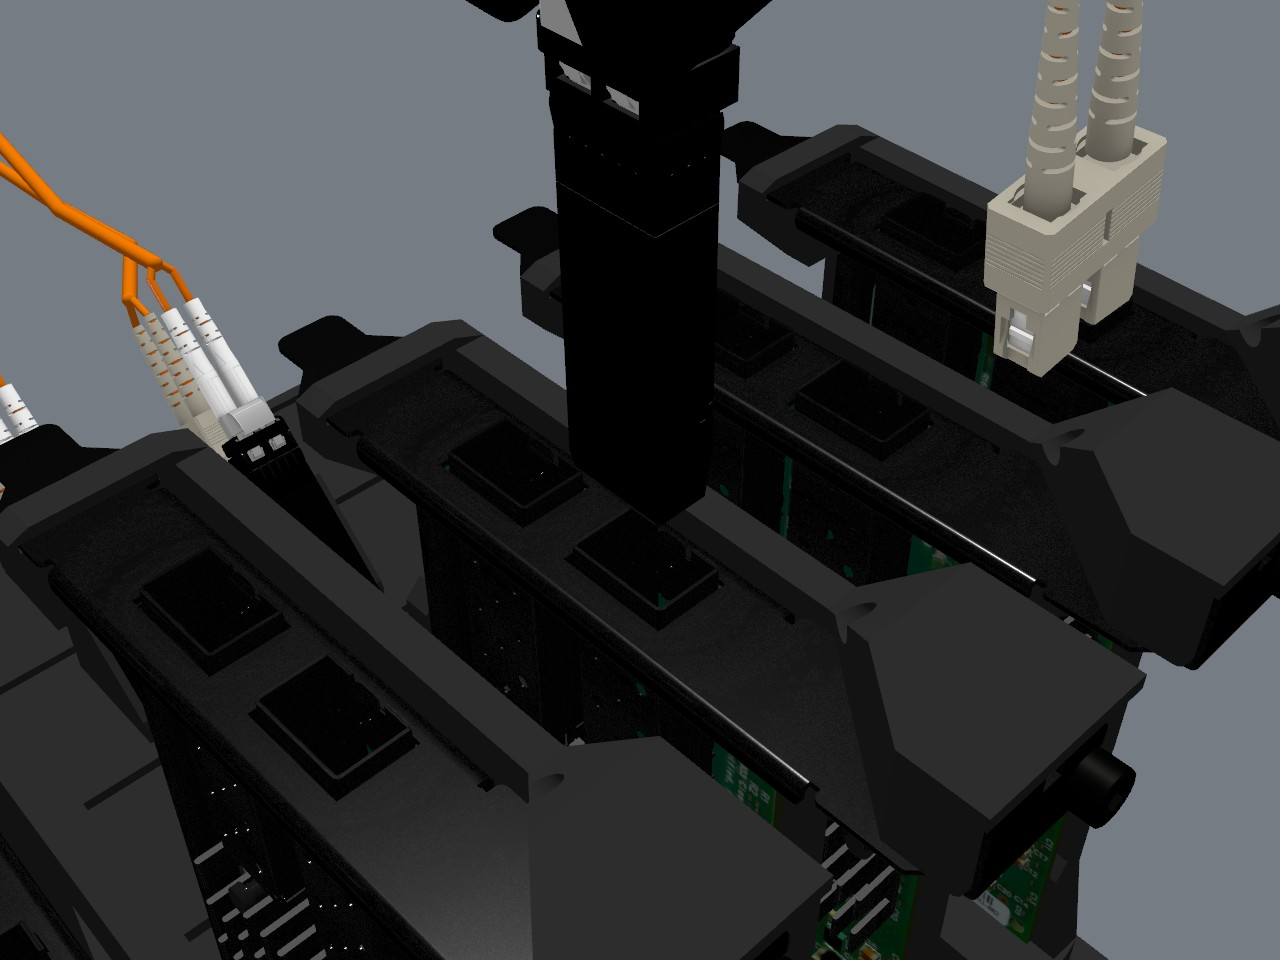
\includegraphics[width=.485\columnwidth]{figures/sfp_before.jpg}&
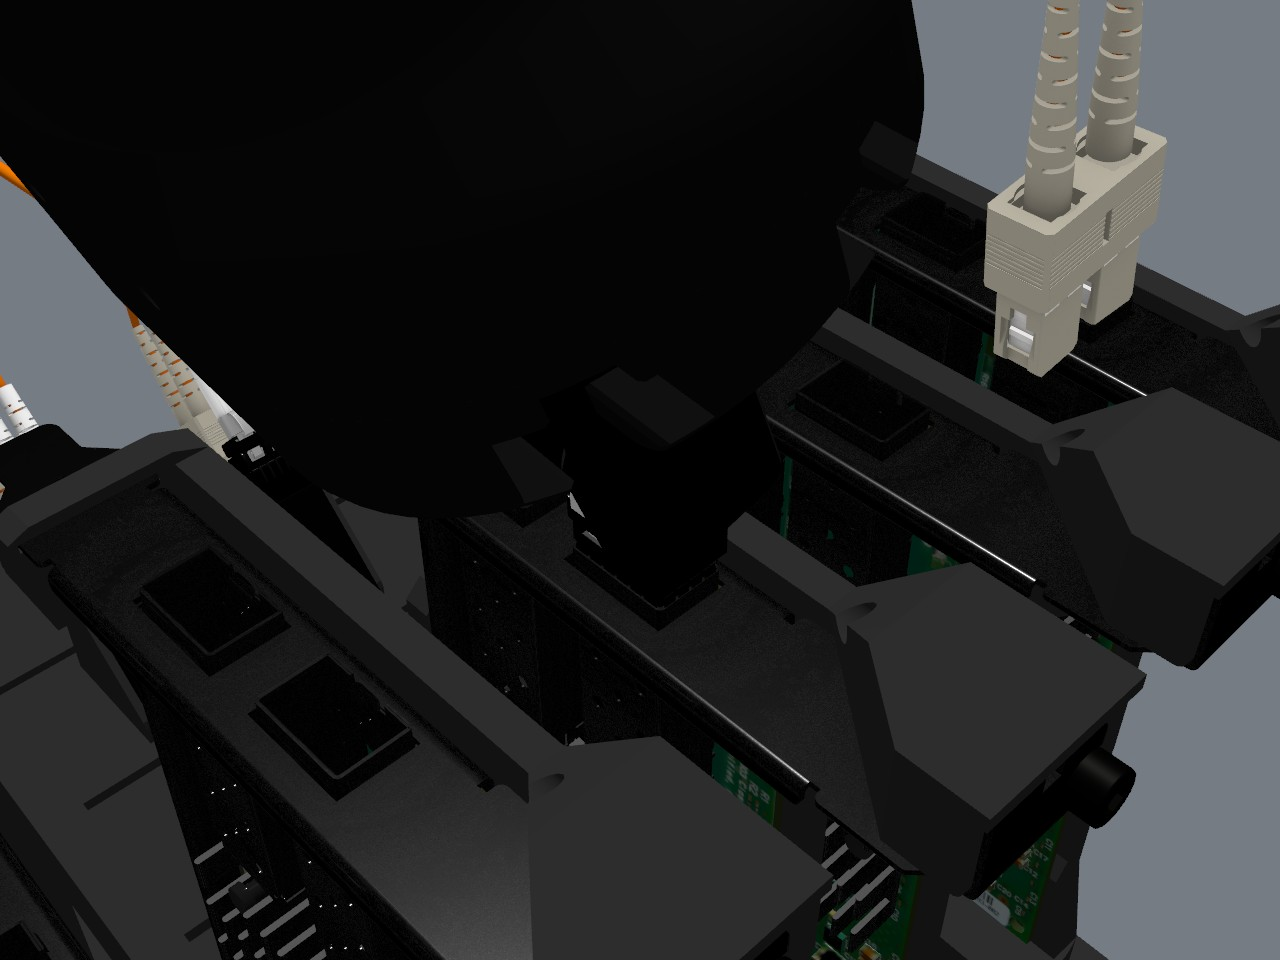
\includegraphics[width=.485\columnwidth]{figures/sfp_after.jpg}\\[-2pt]
\scriptsize SFP approach&\scriptsize SFP verified seat
\end{tabular}
\caption{Headless target-camera frames from recorded SC case 42000 and SFP
case 45005. Gripper occlusion remains visible; images alone cannot certify
engagement. Independent terminal measurements accompany both sequences.}
\label{fig:camera}
\end{figure}

\section{Visual and contact registration}
\subsection{Visual initialization with exposure-time transforms}
Three calibrated wrist cameras provide learned plug and port keypoints~\cite{team}.
Confidence-weighted triangulation and rigid template fitting initialize the
plug frame; reprojection and shape checks reject inconsistent measurements.
Detector confidence supplies fitting weights, not a calibrated probability of
pose accuracy. The original SC plug checkpoint is retained. The SC mouth and
SFP plug/network-interface-card models are adapted from their original
checkpoints using 20 rendered training scenes and six separate development
scenes per connector, with three views per scene. Recovery training uses
60 epochs, 960-pixel inputs, AdamW at $2\times10^{-4}$, and frozen early layers.
Synthetic labels may use simulator poses offline; runtime observations do not.

Let ${}^{B}T_E(t_i)$ be the robot tool-center-point (TCP) transform at image
exposure $t_i$, and ${}^{B}\widehat T_P(t_i)$ the image-derived plug transform.
The cached grasp estimate is
\begin{equation}
 {}^{E}\widehat T_P=
 ({}^{B}T_E(t_i))^{-1}{}^{B}\widehat T_P(t_i).
 \label{eq:grasp}
\end{equation}
Own-robot kinematics then carry the tip estimate through occlusion. Before
inference and image fitting, the pipeline copies exposure-time transforms
that could otherwise expire from transform history. Missing exposure data
rejects the estimate; a latest-pose substitution is not permitted. Processing must
also preserve wrist stationarity within 0.10 mm and $0.05^\circ$.

For SC, learned associations initialize CAD rim and occlusion-aware body
translation fits. A restricted lateral estimate requires repeat-exposure
agreement and subsequent axial registration; it does not establish full pose.
For SFP, directional image edges refine the public two-port entrance geometry,
including its 23.2 mm pitch, while excluding the held-plug footprint.
The fit uses the level-fixture prior rather than an unrestricted orientation
estimate. Figure~\ref{fig:pipeline} summarizes the measurement boundary.

\begin{figure}[t]
\centering
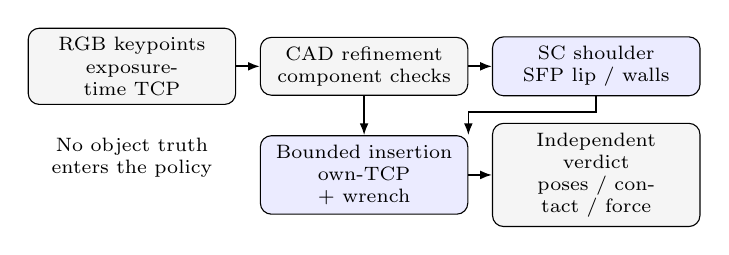
\begin{tikzpicture}[font=\scriptsize, node distance=3mm,
 block/.style={draw,rounded corners,align=center,minimum height=7mm,text width=24mm},
 arr/.style={-{Latex[length=1.5mm]},semithick}]
\node[block,fill=gray!8] (rgb) {RGB keypoints\\exposure-time TCP};
\node[block,fill=gray!8,right=of rgb] (cad) {CAD refinement\\component checks};
\node[block,fill=blue!8,right=of cad] (datum) {SC shoulder\\SFP lip / walls};
\node[block,fill=blue!8,below=5mm of cad] (control) {Bounded insertion\\own-TCP + wrench};
\node[block,fill=gray!8,right=of control] (verify) {Independent verdict\\poses / contact / force};
\draw[arr] (rgb)--(cad);\draw[arr] (cad)--(datum);
\draw[arr] (datum.south)--++(0,-2mm)-|(control.north east);
\draw[arr] (cad)--(control);\draw[arr] (control)--(verify);
\node[align=center,below=3mm of rgb,text width=24mm] {No object truth\\enters the policy};
\end{tikzpicture}
\caption{Visual estimates initialize relative coordinates; connector-specific
contact observations refine them. Evaluator poses and contact flags are used
only after execution and never feed the production correction.}
\label{fig:pipeline}
\end{figure}

\subsection{Geometry determines the physical datum}
With mouth estimate $\widehat p_M$, tip estimate $\widehat p_P$ and insertion
axis $a$, the controller uses relative depth
$\widehat d=a^\top(\widehat p_P-\widehat p_M)$. A visual depth bias can
persist even when the robot tracks its command. A physical datum registers
this relative coordinate through a separate measurement.

\textit{SC terminal shoulder.} SC offers a repeatable shoulder near 15.64 mm
depth. A bounded load/unload/reload sequence combines command advance,
stationary measured motion, compression, release, and repeated stop positions.
The two stop measurements must agree within 0.05 mm, and the applied axial
correction is bounded by 0.5 mm. The legacy SC blocking window requires at
least 20 unique samples over 0.8 s, gaps no greater than 50 ms, and no more
than 25 $\mu$m measured travel. Separate force-noise negative qualification
remains incomplete; the SC detector is not claimed equivalent to SFP's
controlled-excitation check.

\textit{SFP entrance lip and side walls.} The SFP seat is a clearance region
without an equivalent terminal stop. Two probes at opposed $\pm2$ mm lateral
offsets touch the entrance lip; their consistency registers the axial origin
against a public 53.5 $\mu$m datum. Kinematic blocking only triggers the test.
A fixed 0/1/0 N excitation must produce a distinguishable reaction and
subsequent release while the apparent contact location remains stationary.
For load-window means $\bar f_L,\bar f_H$ and standard errors $s_L,s_H$,
\begin{equation}
 \bar f_H-\bar f_L\ \geq\
 \max\!\left(0.025\ \mathrm{N},\;3\sqrt{s_L^2+s_H^2}\right).
 \label{eq:contact}
\end{equation}
The uncertainty uses at least the known 0.2 N per-axis noise floor. Release
must resolve a decrease and return to baseline. Each force window spans
0.4 s, uses actual unique sensor timestamps, and rejects gaps, stale samples,
or tip displacement above 25 $\mu$m. Retained bounded search intent cannot
replace these current measurement checks. Shallow opposed side-wall probes
then register lateral centering before full-depth travel.

\subsection{Bounded execution}
The estimated tip target is converted to a TCP command using
Eq.~\ref{eq:grasp}. Cartesian impedance, persistent depth setpoints, bounded
lateral proportional-integral compensation, and terminal braking reduce
tracking error. Compensation integrates own-robot error, freezes during
contact measurements, and has bounded authority. The evaluated SFP profile
requests 10 mm/s travel and 2 mm/s near the seat, with a 3 N travel pause and
6 N inner abort. The separate 20 N measured resultant ceiling is verified
from raw data; a lower-rate pre-command guard cannot guarantee that bound.
The faster development candidate is not included in the reported cohort.

\section{Testbed and independent verification}
The scene uses public Phase 1 assets~\cite{aic}, pinned at revision 7148df9:
five network-interface cards with two SFP slots each, five SC duplex mounts,
staging fixtures, source cables, a UR5e arm, and an ATI force/torque sensor.
Original visual and collision meshes remain active. A declared rigid grasp
attachment replaces upstream manipulation; automatic port attachment is
disabled. A source-audited double-precision Bullet backend runs at 0.5 ms
with 200 solver iterations and declared cable-joint damping. These are
simulation model choices, not measurements of physical connector compliance.

Before policy execution, a calibrated hold checks reset accuracy, contact
health, and six camera streams. Production inputs are RGB, camera calibration,
exposure-time own-robot transforms, kinematics, public geometry, and wrist
wrench. Object poses, hidden contact state, and scoring signals are excluded
from the policy and retained for diagnostics or independent evaluation only.
Setup failures remain recorded alongside policy failures.

\begin{table}[t]
\caption{Independent continuous terminal dwell criteria}
\label{tab:gates}
\centering\small
\setlength{\tabcolsep}{4pt}
\begin{tabular}{@{}lcc@{}}\toprule
Criterion&SC&SFP\\\midrule
Depth (mm)&$15.64\pm0.25$&$45.80\pm0.25$\\
Maximum lateral error (mm)&0.25&0.10\\
Maximum full angular error (deg)&0.25&0.10\\
Continuous dwell (s)&1.0&1.0\\
Observed penetration limit (mm)&0.10&0.10\\
Every-step wrist force (Hz)&2,000&2,000\\\bottomrule
\end{tabular}
\end{table}

The evaluator applies Table~\ref{tab:gates} to actual simulator poses and
checks the requested target and healthy contact observations. SC additionally
requires terminal physical seating contact. Positive-gap cached manifolds
with zero solver impulse do not suffice. SFP's clearance seat requires both
source-geometry non-overlap and an independently executed deliberate lateral
miss with the identical collision contract, backend, time step, and solver
settings. Surviving control traces were requalified after recovery and contain
1,236 physical contact pairs; their 8.11 N force abort is a positive contact
control, not a successful insertion. All completed policy trials require
complete 2,000 Hz raw wrist coverage. Penetration is evaluated from recorded
contact observations, not proved bounded at every unrecorded instant.

\section{Measured development results}
\subsection{Recovered-policy snapshot}
We freeze the adapted checkpoint hashes, controller sources, and measurement
profiles before replaying predefined development handoffs across target
identities. Table~\ref{tab:results} is an immutable partial snapshot before
speed tuning. The newly trained checkpoints define this measured cohort;
earlier success counts are not pooled with it. Reused development cases and
shared simulation seeds with distinct grasp conditions must not be
interpreted as independent held-out reliability samples.

\begin{table}[t]
\caption{Recovered development snapshot; successful-only median times}
\label{tab:results}
\centering\small
\begin{tabular}{@{}p{43mm}rr@{}}\toprule
Measure&SC&SFP\\\midrule
Verified / completed policy trials&\SCVerified/\SCEligible&\SFPVerified/\SFPEligible\\
Verified / all setup attempts&\SCVerified/\SCAttempts&\SFPVerified/\SFPAttempts\\
Median simulation time (s)&\SCMedianSim&\SFPMedianSim\\
Median wall time (s)&\SCMedianWall&\SFPMedianWall\\
Maximum raw tared force (N)&\SCPeakForce&\SFPPeakForce\\
2,000 Hz force coverage&all&all\\\bottomrule
\end{tabular}
\end{table}

The SFP attempt denominator includes one controller-bootstrap timeout and its
subsequent policy retry. That retry rejected a 2.393 px rim residual against
the unchanged 2 px gate before insertion. The SC setup denominator includes
one duplicate setup cancelled before policy execution after a
resume-bookkeeping error. All attempts remain in the trial ledger.
The snapshot has six distinct attempted case identities per connector; SC
includes shared-seed cases with different grasp conditions. Descriptive Wilson
intervals over completed policy trials are \SCInterval\% for SC and
\SFPInterval\% for SFP. They quantify small-count uncertainty, not population
robustness. The remaining predefined replay cases are pending.

Representative independently verified seats provide a geometric cross-check
beyond the controller's own depth estimate. SC case 42000 remained near
15.566 mm depth with at most 0.1204 mm lateral error and
$0.1346^\circ$ angular error. Its raw peak was 3.322 N. SFP case 45005
remained at 45.805--45.816 mm depth, with 0.0046 mm lateral and
$0.0202^\circ$ angular error; its raw peak was 3.107 N. Their camera
sequences appear in Fig.~\ref{fig:camera}; Fig.~\ref{fig:traces} uses evaluator
traces to show the approach and terminal depth.

\begin{figure}[t]
\centering
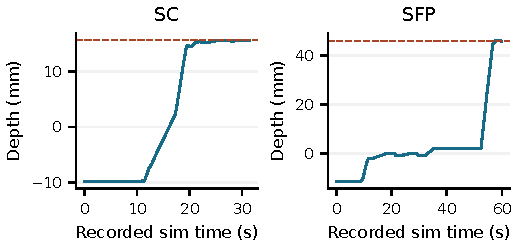
\includegraphics[width=\columnwidth]{figures/depth_traces.pdf}
\caption{Recorded evaluator depth relative to the actual mouth, plotted from
the first recorded sample. Dashed lines mark nominal seats. These diagnostic
poses never enter the production policy. Each final verdict also requires
continuous dwell, alignment, contact validity, and raw-force coverage.}
\label{fig:traces}
\end{figure}

\subsection{What failed and which changes helped}
An earlier matched SC component screen isolates two ingredients under the
same upstream-aligned condition (Table~\ref{tab:ablation}). On five fixed
development cases, removing image-based body translation or lateral tracking
eliminated verified seats. That revision predates current axial registration
and the recovered checkpoints. It supports those components on that screen;
it does not establish the current combined method's causal advantage.

\begin{table}[t]
\caption{Earlier SC revision: five matched development cases}
\label{tab:ablation}
\centering\small
\begin{tabular}{@{}lr@{}}\toprule
Method&Verified / attempted\\\midrule
Body refinement + lateral tracking&5/5\\
Without body translation refinement&0/5\\
Without lateral tracking compensation&0/5\\\bottomrule
\end{tabular}
\end{table}

Failure analysis also exposed errors outside the contact controller. In an
earlier SFP cohort, three of ten trials failed before motion because their
exposure-time transforms expired during computation. Retaining copied
transforms before inference repaired all three selected failures and preserved
one earlier pass: 4/4 under unchanged scoring, with raw peaks 2.9993--3.1833 N.
These selected repairs form a separate cohort and are not pooled into
Table~\ref{tab:results}. Likewise, preserving executed search intent repaired
a sampling-gap failure in probe readiness, but did not relax the sensor
windows needed to accept contact.

The recovered SFP case 45005 took 57.458 simulated and 715.483 wall seconds.
Its final stroke accounted for only 6.96 simulated seconds; the policy's
travel samples peaked at 1.412 N and never reached the 3 N pause. Perception,
approach, and registration therefore dominate this example's cycle time.
Whole-action raw peaks and these lower-rate travel observations are distinct
measurements. Raising a force ceiling alone would not accelerate an
unpaused, velocity-limited stroke. A matched faster-motion study is planned;
no faster-profile outcome or hardware throughput advantage is claimed.

\balance
\section{Discussion and conclusion}
Connector geometry determines which physical datum is available. A terminal
shoulder supports SC axial registration; SFP instead needs an entrance datum
and shallow lateral contacts. The proposed allocation makes those assumptions
and acceptance checks explicit while preserving the original learned,
confidence-weighted visual initialization. Independent verification prevents
estimated depth or command completion from being mistaken for a physical seat.

The frozen snapshot contains six verified SC seats and five SFP seats, with
one SFP perception rejection, one startup failure and a cancelled duplicate
setup retained. All completed
policy trials satisfy the raw-force coverage audit. Earlier SC component
removals and transform-expiry repairs motivate the design, while broader
causal and reliability claims remain open.

The study is simulation-only and conditional on a rigid grasp, upstream
angular alignment, and the SFP fixture prior. It establishes held geometric
seating, not electrical mating, latch retention, cable grasp robustness, or
hardware transfer. \pending{current axial-correction and tracking ablations;
50 fresh SC and 50 fresh SFP trials after development selection and a source/
checkpoint freeze.} Those trials will report all-selected denominators,
failure causes, confidence intervals, and separate simulation/wall times.

\bibliographystyle{IEEEtran}
\bibliography{ref}
\end{document}
